%-------------------------
% Resume in Latex
% Based on: https://github.com/jakegut/resume (which was itself based on https://github.com/sb2nov/resume)
% License : MIT
%------------------------

\documentclass[a4paper,11pt]{article}

\usepackage{latexsym}
\usepackage[empty]{fullpage}
\usepackage{titlesec}
\usepackage{marvosym}
\usepackage[usenames,dvipsnames]{color}
\usepackage{verbatim}
\usepackage{enumitem}
\usepackage[hidelinks]{hyperref}
\usepackage{fancyhdr}
\usepackage[english]{babel}
\usepackage{tabularx}
\usepackage{fontawesome5}
\usepackage[nodayofweek]{datetime}
\usepackage{multicol}
\usepackage[dvipsnames svgnames x11names]{xcolor} % Paquete para el manejo de colores
\usepackage{pagecolor} % Paquete para cambiar el color de fondo de la página
\usepackage[T1]{fontenc}
%\usepackage{lmodern}
\usepackage{pdfpages}



\input{glyphtounicode}

% -------------------- FONT OPTIONS --------------------
% sans-serif
% \usepackage[sfdefault]{roboto}
% \usepackage[sfdefault]{noto-sans}
% serif
% \usepackage{charter}

\pagestyle{fancy}
\fancyhf{} % clear all header and footer fields
\fancyfoot{}
\renewcommand{\headrulewidth}{0pt}
\renewcommand{\footrulewidth}{0pt}

% Adjust margins
\addtolength{\oddsidemargin}{-0.5in}
\addtolength{\evensidemargin}{-0.5in}
\addtolength{\textwidth}{1in}
\addtolength{\topmargin}{-1in} % Default was -.5in
\addtolength{\textheight}{1.0in}

\urlstyle{same}

\raggedbottom
\raggedright
\setlength{\tabcolsep}{0in}

% Section formatting
\titleformat{\section}{
  \vspace{-5pt}\scshape\raggedright\large
}{}{0em}{}[\color{black}\titlerule \vspace{-5pt}]

% Subsection formatting
\titleformat{\subsection}{
  \vspace{-4pt}\scshape\raggedright\large
}{\hspace{-.15in}}{0em}{}[\color{black}\vspace{-8pt}]

% Ensure that generate pdf is machine readable/ATS parsable
\pdfgentounicode=1

% -------------------- CUSTOM COMMANDS --------------------
\newcommand{\resumeItem}[1]{
  \item\small{
    {#1 \vspace{-2pt}}
  }
}

\newcommand{\resumeSubheading}[4]{
  \vspace{-2pt}\item
    \begin{tabular*}{0.97\textwidth}[t]{l@{\extracolsep{\fill}}r}
      \textbf{#1} & #2 \\
      \textit{\small#3} & \textit{\small #4} \\
    \end{tabular*}\vspace{-7pt}
}

\newcommand{\resumeSubSubheading}[2]{
    \item
    \begin{tabular*}{0.97\textwidth}{l@{\extracolsep{\fill}}r}
      \textit{\small#1} & \textit{\small #2} \\
    \end{tabular*}\vspace{-7pt}
}

\newcommand{\resumeProjectHeading}[2]{
    \item
    \begin{tabular*}{0.97\textwidth}{l@{\extracolsep{\fill}}r}
      \small#1 & #2 \\
    \end{tabular*}\vspace{-7pt}
}

\newcommand{\resumeSubItem}[1]{\resumeItem{#1}\vspace{-4pt}}
\newcommand{\resumeSubHeadingListStart}{\begin{itemize}[leftmargin=0.05in, label={}]}
\newcommand{\resumeSubHeadingListEnd}{\end{itemize}}
\newcommand{\resumeItemListStart}{\begin{itemize}}
\newcommand{\resumeItemListEnd}{\end{itemize}\vspace{-5pt}}

\renewcommand\labelitemii{$\vcenter{\hbox{\tiny$\bullet$}}$}

\setlength{\footskip}{4.1pt}

% -------------------- START OF DOCUMENT --------------------
\begin{document}
% -------------------- HEADING--------------------
\begin{flushright}
  % \vspace{-4pt}
  \color{gray}
  \item
  Last Updated on \today
\end{flushright}

\vspace{-4pt}

\begin{center}
    
    \textbf{\Huge \scshape Francisco Concetti} \\ \vspace{4pt}
    \medskip 
    \textbf{\Large \scshape Est. Ingeniería Electrónica} \\ \vspace{4pt}
    \medskip
    \faIcon{envelope}
    \href{mailto:franconcetti16@gmail.com}
    {franconcetti16@gmail.com}    
    \hspace{0.25cm} 
    \faIcon{mobile-alt} 
    \href{tel:+5492914739890}{+54 9 291-473 9890}      
    \hspace{0.25cm}    
    \faIcon{linkedin}
    \href{https://www.linkedin.com/in/francisco-concetti-5258b7232/}{{linkedin.com/in/fconcetti}}
    \hspace{0.25cm}    
    \faIcon{home} 
    {Bahía Blanca} $  $
    %\hspace{1pt}
    \vspace{1pt}
\end{center}

% -------------------- Personal presentation -------------------- 

\section{Presentación Personal}

%Soy estudiante avanzado de Ingeniería Electrónica, actualmente desarrollando mi tesis de grado. Tengo experiencia en sistemas embebidos, automatización y soporte técnico en entornos industriales, adquirida durante mi pasantía en Ternium. Complemento mi perfil con participación en proyectos de diseño digital y programación, así como actividades de voluntariado en Fundación Sí, donde brindo apoyo en matemáticas a estudiantes universitarios. Estas experiencias han fortalecido mis habilidades técnicas, de comunicación y trabajo en equipo. Busco oportunidades para seguir creciendo profesionalmente y aplicar mis conocimientos en un entorno desafiante e innovador.

Soy estudiante avanzado de Ingeniería Electrónica, actualmente finalizando mi tesis de grado y residiendo en Bahía Blanca. Poseo experiencia en entornos industriales a través de mi pasantía en Ternium, donde colaboré en automatización, soporte técnico, diagnóstico y resolución de fallas en sistemas productivos. También participé en tareas de instalación, calibración y mantenimiento de equipos, lo que me permitió adquirir una visión práctica de los procesos de planta.
Mi labor como voluntario en Fundación Sí me brindó la oportunidad de potenciar habilidades de comunicación, escucha activa y trabajo en equipo, competencias que considero fundamentales para un área de mantenimiento.

%Ingeniero Electrónico junior con experiencia práctica en sistemas embebidos, automatización industrial y análisis de datos. He trabajado en entornos productivos reales como Ternium y Marpatech, desarrollando soluciones orientadas a la mejora de procesos. Poseo conocimientos en Python, C/C++, SCADA, PLCs (SIEMENS), así como experiencia en proyectos de inteligencia artificial aplicada. Busco oportunidades en desarrollo embebido, instrumentación o automatización industrial.

%Soy Ingeniero Electrónico junior, actualmente trabajando en mi tesis de grado, con experiencia en diseño digital, automatización y sistemas embebidos. Trabajé en entornos industriales como la planta de Ternium, donde estuve involucrado en tareas de control y soporte técnico. Poseo conocimientos en redes, herramientas colaborativas, y estoy familiarizado con dispositivos Apple y Android. Me destaco por mi proactividad, autonomía y capacidad para adaptarme a nuevos desafíos. Tengo muchas ganas de integrarme a un equipo de trabajo dinámico, seguir aprendiendo y aportar valor desde lo técnico y lo humano. Estoy disponible full time y con gran motivación para desarrollarme profesionalmente.
% -------------------- EDUCATION --------------------
\section{Educación}
  \resumeSubHeadingListStart
    \resumeSubheading
      {Universidad Nacional del Sur}{Bahía Blanca, BsAs}
      {Ingeniería Electrónica - 97\% de aprobación}{MAR 2017 -- Actualidad}
    %\vspace{7pt}
    %\resumeSubheading
      %{Colegio Secundario Don Bosco}{Bahía Blanca, BsAs}
      %{Bachiller en Ciencias Sociales}{2011 -- 2016}
  %\resumeSubHeadingListEnd
\resumeSubHeadingListEnd
% -------------------- EXPERIENCE --------------------
\section{Experiencia}
  \resumeSubHeadingListStart

    %\resumeSubheading
    %{Auxiliar de mantenimiento}{EN 2024 -- ABR 2024}
    %{ESMAR - Cobertura de puesto}{Bahía Blanca, BsAs}
    %\resumeItemListStart
        %\resumeItem{\textbf{Implementé y supervisé} obras de montaje de electricidad e instrumentación, garantizando la entrega dentro de los plazos y presupuestos establecidos.}
        %\resumeItem{\textbf{Gestioné} el mantenimiento de instalaciones de potencia e instrumentación, logrando una reducción en tiempos de inactividad.}
        %\resumeItem{\textbf{Coordiné} proyectos de ampliación y mejoras que resultaron en un aumento de la eficiencia operativa.}
    %\resumeItemListEnd

    \resumeSubheading
    {Practicas Educativas de Verano}{ENE 2025 -- MAR 2025}
    {TERNIUM - Área de operaciones}{San Nicolas de los Arroyos, BsAs}
    \resumeItemListStart
        \resumeItem{Colaboré con ingeniería industrial en la homologación de curvas de calentamiento en Recocido I y II.}
        \resumeItem{Analicé diferencias entre curvas reales y estándar para mejorar su eficiencia.}
        \resumeItem{Estudié la lógica de bobinado/debobinado para proponer mejoras.}
        \resumeItem{Evalué estrategias operativas y sugerí optimizaciones.}
        \resumeItem{Investigué causas de defectos en bobinas en estañado, proponiendo soluciones para mejorar calidad.}
    \resumeItemListEnd

    \resumeSubheading
    {División de Ingenieria y Proyectos}{OCT 2024 - DIC 2024}
    {Marpatech - Ingeniero Electrónico}{CABA, BsAs}
    \resumeItemListStart
        %\resumeItem {Brindé soporte técnico especializado a clientes en la selección y uso de instrumentos de medición y calibración.}
        \resumeItem{Instalación, puesta en marcha y mantenimiento preventivo/correctivo de equipos.}
        \resumeItem{Participé en el proceso de ventas ofreciendo asesoramiento técnico y detallado a los clientes.}
        \resumeItem{Realicé trabajos de campo, incluyendo la instalación, puesta en marcha y calibración de equipos de medición.}
        \resumeItem{Dicté charlas y capacitaciones a clientes sobre el uso adecuado y mantenimiento de los equipos.}
        %\resumeItem{Proveí servicios de mantenimiento preventivo y correctivo para asegurar el óptimo funcionamiento de los instrumentos.}
    \resumeItemListEnd
    \textit{Finalización del proyecto por problemas de salud del dueño y jefe.}

    %\resumeSubheading
    %{Pasante en programación}{NOV 2023 -- DIC 2023}
    %{Alliansys - Movilidad académica ERASMUS+}{CABA, BsAs}
    %\resumeItemListStart
        %\resumeItem{Desarrollé y probé soluciones tecnológicas innovadoras utilizando microcontroladores de Nordic Semiconductor.}
        %\resumeItem{Digitalicé y actualicé bases de datos de proyectos, lo que permitió un acceso más rápido a la información}
        %\resumeItem{Optimicé procesos asignados mediante la automatización de tareas repetitivas, incrementando la eficiencia operativa.}
        %\resumeItem{Asistí en la recopilación de información y documentación para proyectos clave, asegurando la precisión y coherencia en las etapas iniciales de planificación.}
        %\resumeItem{Fortalecí mi capacidad para trabajar en equipo y optimizar flujos de trabajo utilizando herramientas de desarrollo colaborativo.}
        %\resumeItem{}
    %\resumeItemListEnd

    %\resumeSubheading
    %{Asistente de procesos y soporte técnico}{JUL 2023 -- NOV 2023}
    %{Cooperativa Obrera - Convenio Universitario}{Bahía Blanca, BsAs}
    %\resumeItemListStart
        %\resumeItem{Analicé y mejoré procesos operativos, eliminando cuellos de botella y aumentando la productividad del equipo.}
        %\resumeItem{Redacté y mantuve documentación técnica esencial para la operación diaria, garantizando la claridad y accesibilidad de la información técnica.}
        %\resumeItem{Resolví incidentes de hardware y software de manera eficiente, reduciendo los tiempos de inactividad y mejorando la satisfacción del usuario final.}
    %\resumeItemListEnd

    \resumeSubHeadingListEnd
% -------------------- PROJECTS --------------------
\section{Proyectos y Participaciones}
    \resumeSubHeadingListStart

        \resumeProjectHeading
        {\textbf{ECODOC Dental} $|$ \footnotesize\emph{Programación \& entrenamiento de AI para clasificación de imágenes}}{JUL 2024 - DIC 2024}
        \resumeItemListStart
            \begin{multicols}{3}
            \resumeItem{}Implementación de nuevas bases de datos para entrenamiento de IA.
            \resumeItem{Automatización del proceso de identificación de piezas dentales.}            
            \resumeItem{Gestión de proyectos, coordinando equipos y recursos a cargo.}     
            \end{multicols}
          \resumeItemListEnd

        %\resumeProjectHeading
        %{\textbf{PFI-CONICET} $|$ \footnotesize\emph{Entrenamiento de IA para clasificación de imágenes}}{JUL 2023 - MAR 2024}
        %\resumeItemListStart
            %\begin{multicols}{3}
            %\resumeItem{Optimización del proceso de etiquetado de imágenes.}
            %\resumeItem{Desarrollo y entrenamiento de modelos predictivos.}
            %\resumeItem{Creación y organización de datasets estructurados.}     
            %\end{multicols}
        %\resumeItemListEnd

      %\resumeProjectHeading
        {\textbf{EAMTA} $|$ \footnotesize\emph{Diseño digital básico}}{MAR 2024}
        %\resumeItemListStart
            %\resumeItem{Familiarización con estructuras básicas.}
            %\resumeItem{Desarrollo de un proyecto práctico orientado a la implementación.}            
            %\resumeItem{Desarrollo colaborativo de un proyecto introductorio en diseño lógico digital.}
        %\resumeItemListEnd       
    
        %\resumeProjectHeading
        %{\textbf{ChatBuzz} $|$ \footnotesize\emph{TypeScript, HTML/CSS, Webpack, API (Twitch), Git, Unix Shell, VS Code}}{May 2023 -- Present}
        %\resumeItemListStart
            %\resumeItem{Developed a full-stack web application for Twitch livestreamers to display repeated chat messages on OBS}
            %\resumeItem{Experimented with Twitch API's OAuth Access Tokens to get chat data from the given channel}
            %\resumeItem{Collaborated with livestreamers to get feedback and suggested features}
            %\resumeItem{Solved problems relating to asynchronous tasks}
          %\resumeItemListEnd
          
      %\resumeProjectHeading
        %{\textbf{FoodDropper} $|$ \footnotesize\emph{Java, Maven, API (Spigot), Git, IntelliJ IDEA}}{Aug. 2022}
        %\resumeItemListStart
            %\resumeItem{Developed a Minecraft server plugin to limit players to one way of replenishing their hunger bar}
            %\resumeItem{Used persistent data containers to save and load data, ensuring that it persists across plugin resets}
            %\resumeItem{Optimized UX e.g. sound design, food drop timing, supplied saturation level, and addressed potential workarounds}
        %\resumeItemListEnd          
    \resumeSubHeadingListEnd
% -------------------- Voluntariado --------------------
\section{Voluntariado}

\resumeSubHeadingListStart
    \resumeProjectHeading
        {\textbf{Fundacion SI} $|$ \footnotesize\emph{Profesor particular de matemática universitaria}}{SEP 2024 - Actualidad}
        \resumeItemListStart     
            \resumeItem{Diseño planes de enseñanza adaptados a las necesidades individuales de los estudiantes.}
        
            \resumeItem{Colaboro con otros voluntarios y educadores en la planificación de actividades.}

            \resumeItem{Utilizo plataformas virtuales para la enseñanza y el seguimiento del progreso de los estudiantes.}   
    \resumeItemListEnd
\resumeSubHeadingListEnd
% -------------------- SKILLS --------------------
\section{Habilidades}
 \begin{itemize}[leftmargin=0.15in, label={}]
    \small{\item{
    
    \textbf{Idiomas: }{Ingles (C1), Francés (A1)} \\
    \medskip
    
    \textbf{Herramientas: }{Paquete Office, PowerBI, PLC y Scada, AutoCAD, Solid Works, Matlab, Git/GitHub, KiCad, Cadence, Visual Studio, LTSpice.}\\
    \medskip 

    \textbf{Lenguajes de programación: }{Python, AMD VIVADO, C/C++, \LaTeX, Pascal.} \\
    \medskip
     
    %\textbf{Herramientas: }{PowerBI, SQL, Office, Matlab, Git/GitHub, LTSpice, KiCad, Visual Studio, Autocad, SCADA}\\
    %\medskip     
     
     %\textbf{Conocimientos: }{Diseño de circuitos analógicos, Desarrollo de sistemas embebidos, Análisis de señales.} 

     %\textbf{Participaciones: }{EAMTA 2024-Diseño digital básico, capacitación en el uso de AMD Vivado.}\\
     }
     }
 \end{itemize}
%\newpage
%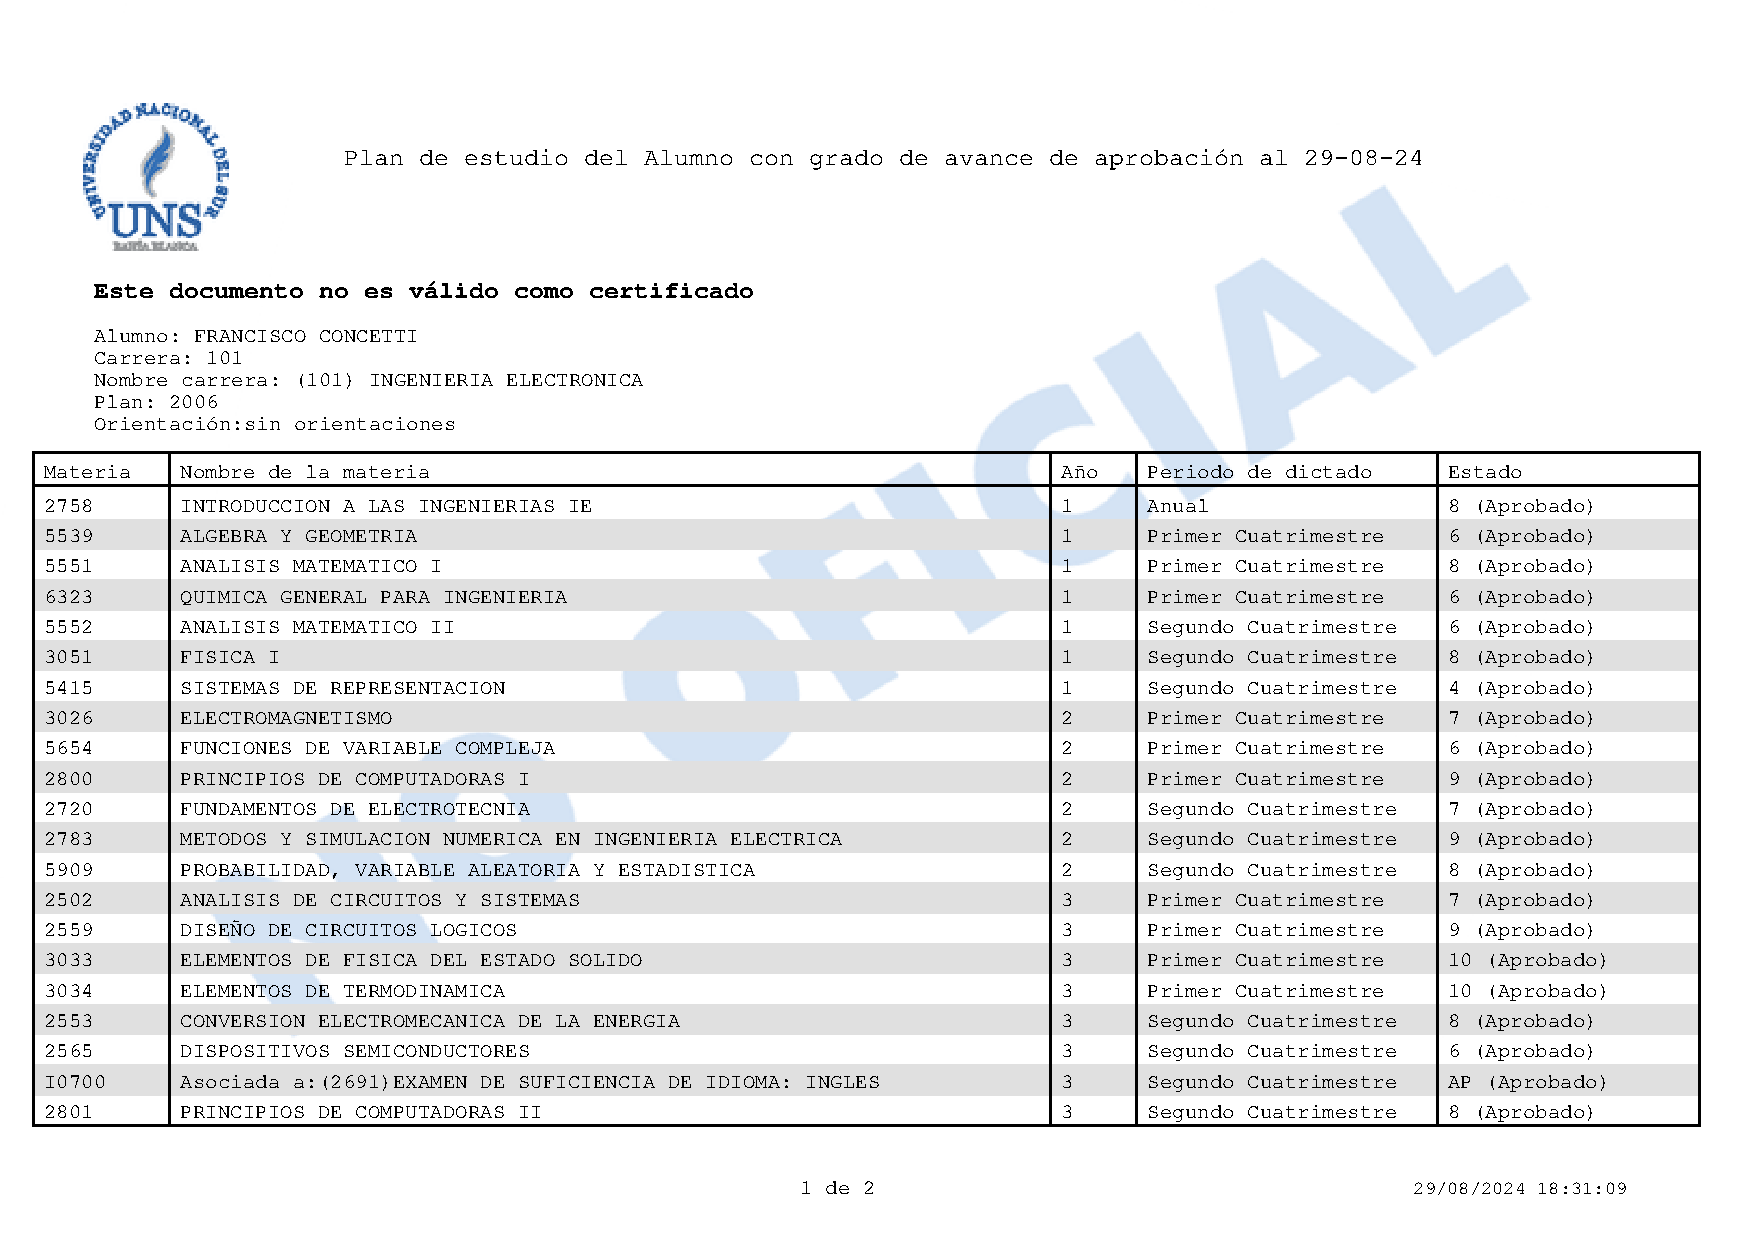
\includepdf[pages=-, angle=90]{Archivos/Analitico.pdf}


\end{document}